%!TEX root = da-dev.tex

In the previous chapter, we studied deterministic distributed algorithms in port-numbered networks. In this chapter we will study a stronger model: \emph{networks with unique identifiers}\mydash see Figure~\ref{fig:unique-ids}. Following the standard terminology of the field, we will use the term ``$\LOCAL$ model'' to refer to networks with unique identifiers.

\begin{figure}
    \centering
    \includegraphics[page=\PUniqueIds]{figs.pdf}
    \caption{A network with unique identifiers.}\label{fig:unique-ids}
\end{figure}


\section{Definitions}\label{sec:unique-id}

Throughout this chapter, fix a constant $c > 1$. An assignment of \emph{unique identifiers} for a port-numbered network $N = (V,P,p)$ is an injection
\[
    \Id \colon V \to \{1,2, \dotsc, |V|^c\}.
\]
That is, each node $v \in V$ is labelled with a unique integer, and the labels are assumed to be relatively small. We will use the shorthand notation $\chi = |V|^c$.

Formally, unique identifiers can be interpreted as a graph problem $\Pi'$, where each solution $\Id \in \Pi'(N)$ is an assignment of unique identifiers for network $N$. If a distributed algorithm $A$ solves a problem $\Pi$ on a family $\calF$ given $\Pi'$, we say that \emph{$A$ solves $\Pi$ on $\calF$ given unique identifiers}, or equivalently, \emph{$A$ solves $\Pi$ on $\calF$ in the $\LOCAL$ model}.

For the sake of convenience, when we discuss networks with unique identifiers, we will identify a node with its unique identifier, i.e., $v = \Id(v)$ for all $v \in V$.


\section{Gathering Everything}\label{sec:gather}

In the $\LOCAL$ model, if the underlying graph $G = (V,E)$ is connected, all nodes can learn everything about $G$ in time $O(\diam(G))$. In this section, we will present algorithm $\algo{Gather}$ that accomplishes this.

In algorithm $\algo{Gather}$, each node $v \in V$ will construct sets $V(v,r)$ and $E(v,r)$, where $r = 1, 2, \dotsc$. For all $v \in V$ and $r \ge 1$, these sets will satisfy
\begin{align}
    V(v,r) &= \ball_G(v,r), \label{eq:gather1} \\
    E(v,r) &= \bigl\{ \{s,t\} : s \in \ball_G(v,r),\, t\in \ball_G(v,r{-}1) \bigr\}. \label{eq:gather2}
\intertext{Now define the graph}
    G(v,r) &= (V(v,r), E(v,r)).  \label{eq:gather3}
\end{align}
See Figure~\ref{fig:gather} for an illustration.

\begin{figure}
    \centering
    \includegraphics[page=\PGather]{figs.pdf}
    \caption{Subgraph $G(v,r)$ defined in \eqref{eq:gather3}, for $v = 14$ and $r = 2$.}\label{fig:gather}
\end{figure}

The following properties are straightforward corollaries of \eqref{eq:gather1}--\eqref{eq:gather3}.
\begin{enumerate}
    \item Graph $G(v,r)$ is a subgraph of $G(v,r+1)$, which is a subgraph of~$G$.
    \item If $G$ is a connected graph, and $r \ge \diam(G) + 1$, we have $G(v,r) = G$.
    \item If $G_v$ is the connected component of $G$ that contains $v$, and $r \ge \diam(G_v) + 1$, we have $G(v,r) = G_v$.
    \item For a sufficiently large $r$, we have $G(v,r) = G(v,r+1)$.
    \item If $G(v,r) = G(v,r+1)$, we will also have $G(v,r+1) = G(v,r+2)$.
    \item Graph $G(v,r)$ for $r > 1$ can be constructed recursively as follows:
    \begin{align}
        V(v,r) &= \bigcup_{u \in V(v,1)} V(u,r-1), \label{eq:Vvr} \\
        E(v,r) &= \bigcup_{u \in V(v,1)} E(u,r-1). \label{eq:Evr}
    \end{align}
\end{enumerate} 

Algorithm $\algo{Gather}$ maintains the following invariant: after round $r \ge 1$, each node $v \in V$ has constructed graph $G(v,r)$. The execution of $\algo{Gather}$ proceeds as follows:
\begin{enumerate}
    \item In round $1$, each node $u \in V$ sends its identity $u$ to each of its ports. Hence after round $1$, each node $v \in V$ knows its own identity and the identities of its neighbours. Put otherwise, $v$ knows precisely $G(v,1)$.
    \item In round $r > 1$, each node $u \in V$ sends $G(u,r-1)$ to each of its ports. Hence after round $r$, each node $v \in V$ knows $G(u,r-1)$ for all $u \in V(v,1)$. Now $v$ can reconstruct $G(v,r)$ using \eqref{eq:Vvr} and \eqref{eq:Evr}.
    \item A node $v \in V$ can stop once it detects that the graph $G(v,r)$ no longer changes.
\end{enumerate}

It is easy to extend $\algo{Gather}$ so that we can discover not only the underlying graph $G = (V,E)$ but also the original port-numbered network $N = (V,P,p)$.


\section{Solving Everything}

Let $\calF$ be a family of connected graphs, and let $\Pi$ be a distributed graph problem. Assume that there is a deterministic \emph{centralised} (non-distributed) algorithm $A'$ that solves $\Pi$ on $\calF$. For example, $A'$ can be a simple brute-force algorithm\mydash we are not interested in the running time of algorithm~$A'$.

Now there is a simple distributed algorithm $A$ that solves $\Pi$ on $\calF$ in the $\LOCAL$ model. Let $N = (V,P,p)$ be a port-numbered network with the underlying graph $G \in \calF$. Algorithm $A$ proceeds as follows.
\begin{enumerate}
    \item All nodes discover $N$ using algorithm $\algo{Gather}$ from Section~\ref{sec:gather}.
    \item All nodes use the centralised algorithm $A'$ to find a solution $f \in \Pi(N)$. From the perspective of algorithm $A$, this is merely a state transition; it is a local step that requires no communication at all, and hence takes $0$ communication rounds.
    \item Finally, each node $v \in V$ switches to state $f(v)$ and stops.
\end{enumerate}
Clearly, the running time of the algorithm is $O(\diam(G))$.

It is essential that all nodes have the same canonical representation of network $N$ (for example, $V$, $P$, and $p$ are represented as lists that are ordered lexicographically by node identifiers and port numbers), and that all nodes use the same deterministic algorithm $A'$ to solve $\Pi$. This way we are guaranteed that all nodes have locally computed the \emph{same} solution $f$, and hence the outputs $f(v)$ are globally consistent.


\section{Focus on Computational Complexity}

So far we have learned the key difference between $\PN$ and $\LOCAL$ models: while there are plenty of graph problems that cannot be solved at all in the $\PN$ model (recall the discussion in Section~\ref{sec:intro-challenges}), we know that all computable graph problems can be easily solved in the $\LOCAL$ model.

Hence our focus shifts from computability to computational complexity. While it is trivial to determine if a problem can be solved in the $\LOCAL$ model, we would like to know which problems can be solved quickly. In particular, we would like to learn which problems can be solved in time that is much smaller than $\diam(G)$. It turns out that graph colouring is an example of such a problem.

In the rest of this chapter, we will design an efficient distributed algorithm that finds a graph colouring in the $\LOCAL$ model. The algorithm will find a proper vertex colouring with $\Delta+1$ colours in $O(\Delta^2 + \log^* |V|)$ communication round, for any graph of maximum degree $\Delta$. We will first present some simpler algorithms that will be used as subroutines\mydash many of these are generalisations and variants of algorithms $\algo{P3C}$ and $\algo{P3CBit}$ that we saw in Chapter~\ref{ch:intro-pos}.


\longsection{Algorithm \talgo{BDGreedy}}{Colour Reduction in Bounded-Degree Graphs}\label{sec:bdgreedy}

Let $x \in \NN$. We present an algorithm called $\algo{BDGreedy}$ that reduces the number of colours from $x$ to
\[
    y = \max \{ x-1, \Delta+1 \},
\]
where $\Delta$ is the maximum degree of the graph. That is, given a proper vertex colouring with $x$ colours, the algorithm outputs a proper vertex colouring with $y$ colours. The running time of the algorithm is one communication round.

\subsection{Algorithm}

The algorithm proceeds as follows; here $f$ is the $x$-colouring that we are given as input and $g$ is the $y$-colouring that we produce as output. See Figure~\ref{fig:greedy} for an illustration.
\begin{enumerate}
    \item In the first communication round, each node $v \in V$ sends its colour $f(v)$ to each of its neighbours.
    \item Now each node $v \in V$ knows the set
    \[
        C(v) = \{ i : \text{there is a neighbour $u$ of $v$ with $f(u) = i$} \}.
    \]
    We say that a node is \emph{active} if $f(v) > \max C(v)$; otherwise it is \emph{passive}. That is, the colours of the active nodes are local maxima. Let
    \[
        \bar{C}(v) = \{1,2,\dotsc\} \setminus C(v)
    \]
    be the set of \emph{free colours} in the neighbourhood of $v$.
    \item A node $v \in V$ outputs
    \[
        g(v) = \begin{cases}
            f(v) & \text{if $v$ is passive}, \\
            \min \bar{C}(v) & \text{if $v$ is active}.
        \end{cases}
    \]
\end{enumerate}
Informally, a node whose colour is a local maximum re-colours itself with the first available free colour.

\begin{figure}
    \centering
    \includegraphics[page=\PGreedy]{figs.pdf}
    \caption{Greedy colour reduction. The active nodes have been highlighted. Note that in the original colouring $f$, the largest colour was $99$, while in the new colouring, the largest colour is strictly smaller than $99$\mydash we have successfully reduced the number of colours in the graph.}\label{fig:greedy}
\end{figure}

\subsection{Analysis}

\begin{lemma}
    Algorithm $\algo{BDGreedy}$ reduces the number of colours from $x$ to
    \[
        y = \max \{ x-1, \Delta+1 \},
    \]
    where $\Delta$ is the maximum degree of the graph.
\end{lemma}
\begin{proof}
    Let us first prove that $g(v) \in \{1,2,\dotsc,y\}$ for all $v \in V$. As $f$ is a proper colouring, we cannot have $f(v) = \max C(v)$. Hence there are only two possibilities.
    \begin{enumerate}
        \item $f(v) < \max C(v)$. Now $v$ is passive, and it is adjacent to a node $u$ such that $f(v) < f(u)$. We have
        \[
            g(v) = f(v) \le f(u) - 1 \le x - 1 \le y.
        \]
        \item $f(v) > \max C(v)$. Now $v$ is active, and we have
        \[
            g(v) = \min \bar{C}(v).
        \]
        There is at least one value $i \in \{1,2,\dotsc,|C(v)|+1\}$ with $i \notin C(v)$; hence
        \[
            \min \bar{C}(v) \le |C(v)| + 1 \le \deg_G(v) + 1 \le \Delta + 1 \le y.
        \]
    \end{enumerate}
    
    Next we will show that $g$ is a proper vertex colouring of $G$. Let $\{u,v\} \in E$. If both $u$ and $v$ are passive, we have
    \[
        g(u) = f(u) \ne f(v) = g(v).
    \]
    Otherwise, w.l.o.g., assume that $u$ is active. Then we must have $f(u) > f(v)$. It follows that $f(u) \in C(v)$ and $f(v) \le \max C(v)$; therefore $v$ is passive. Now
    $g(u) \notin C(u)$ while
    $g(v) = f(v) \in C(u)$; we have $g(u) \ne g(v)$.
\end{proof}

The key observation is that the set of active nodes forms an independent set. Therefore all active nodes can pick their new colours simultaneously in parallel, without any risk of choosing colours that might conflict with each other.

\subsection{Remarks}

Algorithm $\algo{BDGreedy}$ does not need to know the number of colours $x$ or the maximum degree $\Delta$; we only used them in the analysis. We can take any graph, blindly apply algorithm $\algo{BDGreedy}$, and we are guaranteed to reduce the number of colours by one\mydash provided that the number of colours was larger than $\Delta + 1$. In particular, we can apply algorithm $\algo{BDGreedy}$ repeatedly until we get stuck, at which point we have a \Dpocol{} of~$G$\mydash we will formalise and generalise this idea in Exercise~\ref{ex:greedy-iterate}.


\section{Directed Pseudoforests}

We will next study graph colouring in so-called directed pseudoforests. As we will see later, algorithms that colour directed pseudoforests can be used as subroutines in algorithms that colour bounded-degree graphs.

A \emph{directed pseudoforest} is a directed graph $G = (V,E)$ such that each node $v \in V$ has $\outdegree_G(v) \le 1$; see Figure~\ref{fig:dp} for an example.

\begin{figure}
    \centering
    \includegraphics[page=\PDP]{figs.pdf}
    \caption{A directed pseudoforest with a colouring~$f$.}\label{fig:dp}
\end{figure}

Compare the definition of a directed pseudoforest with the definition of a \emph{pseudoforest} in Section~\ref{ssec:graphs-conn}. We make the following observations:
\begin{enumerate}
    \item Let $H$ be an undirected graph, and let $G$ be an orientation of $H$. If $G$ is a directed pseudoforest, then $H$ is a pseudoforest.
    \item Let $H$ be a pseudoforest. There exists an orientation $G$ of $H$ such that $G$ is a directed pseudoforest.
    \item An orientation of a pseudoforest is not necessarily a directed pseudoforest.
\end{enumerate}
If $(u,v) \in E$, we say that $v$ is a \emph{successor} of $u$ and $u$ is a \emph{predecessor} of~$v$. By definition, in a directed pseudoforest each node has at most one successor.


\longsection{Algorithm \talgo{DPGreedy}}{Colour Reduction in Directed Pseudoforests}\label{sec:dpgreedy}

Let $G = (V,E)$ be a directed pseudoforest, and let $f$ be a proper vertex colouring of $G$ with $x$ colours, for some $x \ge 4$. We design a distributed algorithm $\algo{DPGreedy}$ that reduces the number of colours from $x$ to $x-1$ in two communication rounds.

Note the key difference between algorithms $\algo{BDGreedy}$ and $\algo{DPGreedy}$: algorithm $\algo{BDGreedy}$ gets stuck at $\Delta+1$ colours, while $\algo{DPGreedy}$ can be used to reduce the number of colours down to~$3$.


\subsection{Overview}

The high-level structure of algorithm $\algo{DPGreedy}$ is as follows:
\begin{enumerate}
    \item We are given an $x$-colouring $f$ (Figure~\ref{fig:dp}).
    \item In one communication round, given $f$ we construct another $x$-colouring $s$, which has the property that each node is adjacent to at most two different colour classes (Figure~\ref{fig:dpsuccessor}).
    \item In one communication round, given $s$ we construct an $(x-\nobreak 1)$-colouring $g$ using algorithm $\algo{BDGreedy}$ (Figure~\ref{fig:dpgreedy}).
\end{enumerate}

\begin{figure}
    \centering
    \includegraphics[page=\PDPSuccessor]{figs.pdf}
    \caption{A directed pseudoforest with colouring~$s$; compare with Figure~\ref{fig:dp}. In colouring $s$, all predecessors of a node have the same colour; hence each node is adjacent to nodes of only two different colours.}\label{fig:dpsuccessor}
\end{figure}

\begin{figure}
    \centering
    \includegraphics[page=\PDPGreedy]{figs.pdf}
    \caption{Algorithm $\algo{BDGreedy}$ applied to a directed pseudoforest with colouring~$s$. The active nodes are highlighted.}\label{fig:dpgreedy}
\end{figure}


\subsection{Algorithm}

First, each $v \in V$ computes $s(v)$ as follows; see Figure~\ref{fig:dpsuccessor}:
\begin{enumerate}
    \item If $\outdegree_G(v) = 1$, let $u$ be the successor of $v$, and let $s(v) = f(u)$.
    \item Otherwise, if $f(v) > 1$, let $s(v) = 1$.
    \item Otherwise $s(v) = 2$.
\end{enumerate}
Then we apply $\algo{BDGreedy}$ from Section~\ref{sec:bdgreedy} to labelling $s$ to construct another labelling $g$.


\subsection{Analysis}

We will first prove that the values $s(v)$ form a proper $x$-colouring of~$G$. Moreover, we will show that each node is adjacent to only two different colours in colouring~$s$.

\begin{lemma}
    Function $s$ is an $x$-colouring of $G$.
\end{lemma}
\begin{proof}
    By construction, we have $s(v) \in \{1,2,\dotsc,x\}$. Now let $(u,v) \in E$. We need to show that $s(u) \ne s(v)$. To see this, observe that $v$ is a successor of $u$. Hence
    \[
        s(u) = f(v) \ne s(v). \qedhere
    \]
\end{proof}

\begin{lemma}
    Define
    \[
        C(v) = \{ i : \text{there is a neighbour $u$ of $v$ with $s(u) = i$} \}.
    \]
    We have $|C(v)| \le 2$ for each node $v \in V$.
\end{lemma}
\begin{proof}
    For each predecessor $u$ of $v$, we have $s(u) = f(v)$. That is, all predecessors of $v$ have the same colour. Hence $C(v)$ consists of at most two different values: the common colour of the predecessors of $v$ (if any), and the colour of the successor of $v$ (if any).
\end{proof}

Now let us consider what happens when we apply algorithm $\algo{BDGreedy}$ to construct labelling $g$. Each active node $v$ will choose a colour \[g(v) = \min \bar{C}(v) \in \{1,2,3\},\] while each passive node $v$ will output its old colour $g(v) = s(v)$. In particular, if the number of colours in $f$ was $x \ge 4$, then the number of colours in $g$ is at most $x - 1$.

We conclude that we have designed algorithm $\algo{DPGreedy}$ that reduces the number of colours from $x \ge 4$ to $x-1$ in directed pseudoforests in $2$ communication rounds. In particular, we can reduce the number of colours from any number $x \ge 3$ to $3$ in ${2(x-3)}$ rounds.


\longsection{Algorithm \talgo{DPBit}}{Fast Colour Reduction in Directed Pseudoforests}\label{sec:dpbit}

So far we have only seen algorithms that reduce the number of colours by one in each iteration. In this section we will present an algorithm that is \emph{much} faster. We present algorithm $\algo{DPBit}$ that reduces the number of colours from $2^x$ to $2x$ in one communication round, in any directed pseudoforest. We will assume that $x \ge 1$ is a known constant. In essence, this is the same algorithm as $\algo{P3CBit}$ from Section~\ref{sec:algo-p3cbit}\mydash fast colour reduction in directed pseudoforests is almost as easy as fast colour reduction in directed paths.

\subsection{Algorithm}

We assume that we are given a proper vertex colouring
\[
    f \colon V \to \{ 1,2,\dotsc,2^x\}
\]    
of a directed pseudoforest $G = (V,E)$. We will use the values $s(v)$ defined in Section~\ref{sec:dpgreedy}\mydash recall that $f(v) \ne s(v)$ for each node $v$, and if $u$ is the successor of $v$, we have $s(v) = f(u)$.

The key idea is that each node compares the \emph{binary encodings} of the values $s(v)$ and $f(v)$. More precisely, if $j \in \{1,2,\dotsc,2^x\}$ is a colour, let us use $\bin{j}$ to denote the binary encoding of $j-1$; this is always a binary string of length $x$. For example, if $x = 3$, we have
\[
    \bin{1} = 000,\quad
    \bin{2} = 001,\quad
    \dotsc, \quad
    \bin{8} = 111.
\]
If $i \in \{0,1,\dotsc,x-1\}$, we use the notation $\bin{j}_i$ to refer to bit $i$ of the binary string $\bin{j}$, counting from the lowest-order bit. For example, $\bin{2}_0 = 1$ and $\bin{2}_1 = 0$.

In algorithm $\algo{DPBit}$, each node first finds out the values $s(v)$ and $f(v)$\mydash this takes only one communication round\mydash and then compares the binary strings $\bin{s(v)}$ and $\bin{f(v)}$. As $s(v) \ne f(v)$, there is at least one bit in these strings that differs. Let
\[
    i(v) = \min \{ i : \bin{f(v)}_i \ne \bin{s(v)}_i \}
\]
be the \emph{index} of the first bit that differs, and let
\[
    b(v) = \bin{f(v)}_{i(v)}
\]
be the \emph{value} of the bit that differs. Note that $0 \le i(v) \le x-1$ and $0 \le b(v) \le 1$. We encode the pair $\bigl(i(v), b(v)\bigr)$ as a colour
\[
    g(v) = 2i(v) + b(v) + 1.
\]
Algorithm $\algo{DPBit}$ outputs the value $g(v)$.

\subsection{Analysis}

The key observation is that the pairs $\bigl(i(v), b(v)\bigr)$ form a proper colouring of $G$.
\begin{lemma}\label{lem:dpbit}
    Let $(u,v) \in E$. We have $i(u) \ne i(v)$ or $b(u) \ne b(v)$.
\end{lemma}
\begin{proof}
    If $i(u) \ne i(v)$, the claim is trivial. Otherwise $i(u) = i(v)$. As $v$ is the successor of $u$, we have $s(u) = f(v)$. Hence
    \begin{align*}
        b(v) &= \bin{f(v)}_{i(v)} = \bin{s(u)}_{i(u)}, \\
    \intertext{and by the definition of $i(u)$,}
        b(u) &= \bin{f(u)}_{i(u)} \ne \bin{s(u)}_{i(u)}.
    \end{align*}
    In summary, $b(u) \ne b(v)$.
\end{proof}

Note that if we have $g(u) = g(v)$ for two nodes $u$ and $v$, this implies $b(u) = b(v)$ and $i(u) = i(v)$. Hence Lemma~\ref{lem:dpbit} implies that $g$ is a proper vertex colouring of $G$. Moreover, we have $1 \le g(v) \le 2x$, and hence $g$ is a $2x$-colouring of $G$.

In summary, we have designed algorithm $\algo{DPBit}$ that reduces the number of colours from $2^x$ to $2x$ in one communication round\mydash given a $2^x$-colouring $f$, the algorithm outputs a $2x$-colouring $g$.


\longsection{Algorithm \talgo{DP3C}}{Fast 3-Colouring in Directed Pseudoforests}\label{sec:dp3c}

Assume that we know $|V|$. We will design algorithm $\algo{DP3C}$ that finds a $3$-colouring in $O(\log^* |V|)$ rounds in any directed pseudoforest. The algorithm proceeds as follows:
\begin{enumerate}
    \item Use the unique identifiers to construct a colouring with $\chi$ colours.
    \item Repeat algorithm $\algo{DPBit}$ for $\log^* \chi$ times to reduce the number of colours from $\chi$ to $6$.
    \item Repeat algorithm $\algo{DPGreedy}$ for $3$ times to reduce the number of colours from $6$ to~$3$.
\end{enumerate}
Here phase~(a) takes $0$ communication rounds, phase~(b) takes $\log^* \chi$ communication rounds, and phase~(c) takes $6$ communication rounds. The analysis is, in essence, identical to what we already did in Exercise~\ref{ex:logstar}.


\longsection{Algorithm \talgo{BDColour}}{Fast Colouring in Bounded-Degree Graphs}\label{sec:bdcolour}

Now we will turn our attention to bounded-degree graphs. Assume that we know $|V|$ and $\Delta$. We will now design a distributed algorithm $\algo{BDColour}$ that finds a $(\Delta+1)$-colouring in any graph of maximum degree at most $\Delta$ in $O(\Delta^2 + \log^* |V|)$ rounds.

\subsection{Preliminaries}

For each node $v$ and each port number $i$, node $v$ sends the pair $(v, i)$ to port $i$. This way a node $u$ learns the following information about each node $v$ that is adjacent to~$u$: what is the unique identifier of $v$, which port of $u$ is connected to $v$, and which port of $v$ is connected to $u$. This step requires one communication round.

\subsection{Orientation}

We construct an orientation $G' = (V,E')$ of $G$ as follows: we have $(u,v) \in E'$ if and only if $\{u,v\} \in E$ and $u < v$. That is, we use the unique identifiers to orient the edges; see Figure~\ref{fig:id-orient}. Each node only needs to know the orientation of its incident edges. This step requires zero communication rounds.

\begin{figure}
    \centering
    \includegraphics[page=\PIdOrient]{figs.pdf}
    \caption{Orientation $G'$ derived from the unique identifiers.}\label{fig:id-orient}
\end{figure}


\subsection{Partition in Pseudoforests}

For each $i = 1,2,\dotsc,\Delta$, we construct a subgraph $G_i = (V,E_i)$ of $G'$ as follows: we have $(u,v) \in E_i$ if and only if $(u,v) \in E'$ and $v$ is connected to port number $i$ of $u$ in $N$. See Figure~\ref{fig:id-pick-class}.

\begin{figure}
    \centering
    \includegraphics[page=\PIdPickClass]{figs.pdf}
    \caption{Subgraph $G_i$ of $G'$. Each node has outdegree at most one.}\label{fig:id-pick-class}
\end{figure}
    
Observe that the sets $E_1, E_2, \dotsc, E_\Delta$ form a partition of $E'$: for each directed edge $e \in E'$ there is precisely one $i$ such that $e \in E_i$. Also note that for each node $u \in V$ and for each index $i$ there is at most one neighbour $v$ such that $(u,v) \in E_i$. It follows that the outdegree of any node $v$ in $G_i = (V,E_i)$ is at most one, and therefore $G_i$ is a \emph{directed pseudoforest}.
    
Each node only needs to know which of its incident edges are in which subset $E_i$. This step requires zero communication rounds.

\subsection{Parallel Colouring of Pseudoforests}

For each $i$, we use algorithm $\algo{DP3C}$ to construct a $3$-colouring $g_i$ of $G_i$. Each node $v \in V$ needs to know the value $g_i(v)$ for each $i$. This step takes only $O(\log^* |V|)$ rounds: we can simulate the execution of $A$ in parallel for all subgraphs $G_i$. In the simulation, each node has $\Delta$ different roles, one for each subgraph $G_i$.

\subsection{Merging Colourings}

For each $j = 0, 1, \dotsc, \Delta$, define
\[
    E'_j = \bigcup_{i = 1}^j E_i
\]
and $G'_j = (V,E'_j)$. Note that $G'_0$ is a graph without any edges, each $G'_j$ is a subgraph of $G'$, and $G'_\Delta = G'$.

We will construct a sequence of colourings $g'_0, g'_1, \dotsc, g'_\Delta$ such that $g'_j$ is a \Dpocol{} of the subgraph $G'_j$. Then it follows that we can output $g = g'_\Delta$, which is a \Dpocol{} of $G'$ and hence also a \Dpocol{} of the original graph~$G$.

Our construction is recursive. The base case of $j = 0$ is trivial: we can choose $g'_0(v) = 1$ for all $v \in V$, and this is certainly a proper \Dpocol{} of $G'_0$.

\begin{figure}
    \centering
    \includegraphics[page=\PMergeColours]{figs.pdf}
    \caption{Merging a $3$-colouring $g_j$ of directed pseudotree $G_j$ and a \Dpocol{} $g'_{j-1}$ of subgraph $G'_{j-1}$. The end result is a proper $3(\Delta\nobreak +1)$-colouring $h_j$ of subgraph $G'_j$.}\label{fig:merge-colours}
\end{figure}

Now assume that we have already constructed a \Dpocol{} $g'_{j-1}$ of $G'_{j-1}$. Recall that $g_j$ is a $3$-colouring of $G_j$; see Figure~\ref{fig:merge-colours}. Define a function $h_j$ as follows:
\[
    h_j(v) = (\Delta+1) (g_j(v)-1) + g'_{j-1}(v).
\]
Observe that $h_j$ is a proper $3(\Delta+\nobreak 1)$-colouring of $G'_j$. To see this, consider an edge $(u,v) \in E'_j$. If $(u,v) \in E_j$, we have $g_j(u) \ne g_j(v)$, which implies $h_j(u) \ne h_j(v)$. Otherwise $(u,v) \in E'_{j-1}$, and we have $g'_{j-1}(u) \ne g'_{j-1}(v)$, which implies $h_j(u) \ne h_j(v)$.

Now we use $2(\Delta+\nobreak 1)$ iterations of $\algo{BDGreedy}$ to reduce the number of colours from $3(\Delta+\nobreak 1)$ to $\Delta+\nobreak 1$. This way we can construct a proper \Dpocol{} $g'_j$ of $G'_j$ in time $O(\Delta)$.

After $\Delta$ phases, we have eventually constructed colouring $g = g'_\Delta$; the total running time is $O(\Delta^2)$, as each phase takes $O(\Delta)$ communication rounds.


\subsection{Summary}

In this section, we have seen how to find a proper vertex colouring with $\Delta+1$ colours in $O(\Delta^2 + \log^* x)$ communication round in the $\LOCAL$ model, for any graph of maximum degree $\Delta$. In the exercises, we will see that efficient algorithms for vertex colouring can be used as subroutines to solve many other problems.


\section{Exercises}

\begin{ex}[applications]
    Let $\Delta$ be a known constant, and let $\calF$ be the family of graphs of maximum degree at most $\Delta$. Design fast distributed algorithms that solve the following problems on $\calF$ in the $\LOCAL$ model.
    \begin{subex}
        \item Maximal independent set.
        \item Maximal matching.
        \item Edge colouring with $O(\Delta)$ colours.
    \end{subex}
    
    \hint{You can either use algorithm $\algo{BDColour}$ as a subroutine, or you can modify the basic idea of $\algo{BDColour}$ slightly to solve these problems.}
\end{ex}

\begin{ex}[vertex cover]
    Let $\calF$ consist of cycle graphs. Design a fast distributed algorithm that finds a \Apx{1.1} of a minimum vertex cover on $\calF$ in the $\LOCAL$ model.
    
    \hint{Solve small problem instances by brute force and focus on the case of long cycles. In a long cycle, use a graph colouring algorithm to find a $3$-colouring, and then use the $3$-colouring to construct a maximal independent set. Observe that a maximal independent set partitions the cycle into short fragments (with 2--3 nodes in each fragment).

    Apply the same approach recursively: interpret each fragment as a ``supernode'' and partition the cycle that is formed by the supernodes into short fragments, etc. Eventually, you have partitioned the original cycle into \emph{long} fragments, with dozens of nodes in each fragment.
    
    Find an optimal vertex cover within each fragment. Make sure that the solution is feasible near the boundaries, and prove that you are able to achieve the required approximation ratio.}
\end{ex}

\begin{ex}[iterated greedy]\label{ex:greedy-iterate}
    Design a colour reduction algorithm $A$ with the following properties:
    given any graph $G = (V,E)$ and any proper vertex colouring~$f$,
    algorithm $A$ outputs a proper vertex colouring~$g$ such that
    for each node $v \in V$ we have $g(v) \le \deg_G(v) + 1$.
    
    Let $\Delta$ be the maximum degree of $G$, let $n = |V|$ be the number of nodes in $G$, and let $x$ be the number of colours in colouring $f$. The running time of $A$ should be at most
    \[
        \min \{ n, x \} + O(1).
    \]
    Note that the algorithm does not know $n$, $x$, or $\Delta$. Also note that we may have either $x \le n$ or $x \ge n$.
    
    \hint{Adapt the basic idea of algorithm $\algo{BDGreedy}$\mydash find local maxima and choose appropriate colours for them\mydash but pay attention to the stopping conditions and low-degree nodes. One possible strategy is this: a node becomes active if its current colour is a local maximum among those neighbours that have not yet stopped; once a node becomes active, it selects an appropriate colour and stops.}
\end{ex}

\begin{ex}[distance-$2$ colouring]\label{ex:distance2col}
    Let $G = (V,E)$ be a graph. A \emph{distance-$2$ colouring with $k$ colours} is a function $f \colon V \to \{1,2,\dotsc,k\}$ with the following property:
    \[
        \dist_G(u,v) \le 2 \text{ implies } f(u) \ne f(v) \text{ for all nodes } u \ne v.
    \]

    Let $\Delta$ be a known constant, and let $\calF$ be the family of graphs of maximum degree at most $\Delta$. Design a fast distributed algorithm that finds a distance-$2$ colouring with $O(\Delta^2)$ colours for any graph $G \in \calF$ in the $\LOCAL$ model.
    
    \hint{Given a graph $G \in \calF$, construct a virtual graph $G^2 = (V, E')$ as follows: $\{u,v\} \in E'$ if $u \ne v$ and $\dist_G(u,v) \le 2$. Prove that the maximum degree of $G^2$ is $O(\Delta^2)$. Simulate a fast graph colouring algorithm on $G^2$.}
\end{ex}

\begin{exs}[numeral systems]\label{ex:dpbit-base}
    Algorithm $\algo{DPBit}$ is based on the idea of identifying a digit that differs in the \emph{binary} encodings of the colours. Generalise the idea: design an analogous algorithm that finds a digit that differs in the base-$k$ encodings of the colours, for an arbitrary $k$, and analyse the running time of the algorithm (cf.\ Exercise~\ref{ex:logstar-tight}). Is the special case of $k = 2$ the best possible choice?
\end{exs}

\begin{exs}[from bits to sets]\label{ex:dpset}
    Algorithm $\algo{DPBit}$ can reduce the number of colours from $2^x$ to $2x$ in one round in any directed pseudoforest, for any positive integer $x$. For example, we can reduce the number of colours as follows:
    \[
        2^{128} \to 256 \to 16 \to 8 \to 6.
    \]
    One of the problems is that an iterated application of the algorithm slows down and eventually ``gets stuck'' at $x = 3$, i.e., at six colours.
    
    In this exercise we will design a distributed algorithm $\algo{DPSet}$ that reduces the number of colours from
    \[
        h(x) = \binom{2x}{x}
    \]
    to $2x$ in one round, for any positive integer $x$. For example, we can reduce the number of colours as follows:
    \[
        184756 \to 20 \to 6 \to 4.
    \]
    Here
    \begin{align*}
        184756 &= h(10), \\
        2 \cdot 10 = 20 &= h(3), \\
        2 \cdot 3 = 6 &= h(2).
    \end{align*}
    In particular, algorithm $\algo{DPSet}$ does not get stuck at six colours; we can use the same algorithm to reduce the number of colours to four. Moreover, at least in this case the algorithm seems to be much more efficient\mydash algorithm $\algo{DPSet}$ can reduce the number of colours from $184756$ to $6$ in two rounds, while algorithm $\algo{DPBit}$ requires at three rounds to achieve the same reduction.
    
    The basic structure of algorithm $\algo{DPSet}$ follows algorithm $\algo{DPBit}$\mydash in particular, we use one communication round to compute the values $s(v)$ for all nodes $v \in V$. However, the technique for choosing the new colour is different: as the name suggests, we will not interpret colours as bit strings but as \emph{sets}.
    
    To this end, let $H(x)$ consist of all subsets
    \[
        X \subseteq \{1,2,\dotsc,2x\}
    \]
    with $|X| = x$. There are precisely $h(x)$ such subsets, and hence we can find a bijection
    \[
        L\colon \{1,2,\dotsc,h(x)\} \to H(x).
    \]
    
    We have $f(v) \ne s(v)$. Hence $L(f(v)) \ne L(s(v))$. As both $L(f(v))$ and $L(s(v))$ are subsets of size $x$, it follows that
    \[
        L(f(v)) \setminus L(s(v)) \ne \emptyset.
    \]
    We choose the new colour $g(v)$ of a node $v \in V$ as follows:
    \[
        g(v) = \min \bigl( L(f(v)) \setminus L(s(v)) \bigr).
    \]

    Prove that $\algo{DPSet}$ works correctly. In particular, show that $g\colon V \to \{1,2,\dotsc,2x\}$ is a proper graph colouring of the directed pseudoforest~$G$.
    
    Analyse the running time of $\algo{DPSet}$ and compare it with $\algo{DPBit}$. Is $\algo{DPSet}$ always faster? Can you prove a general result analogous to the claim of Exercise~\ref{ex:logstar-tight}?
\end{exs}

\begin{exs}[dominating set approximation]\label{ex:greedy-domset}
    Let $\Delta$ be a known constant, and let $\calF$ be the family of graphs of maximum degree at most $\Delta$. Design an algorithm that finds an \Apx{O(\log \Delta)} of a minimum dominating set on $\calF$ in the $\LOCAL$ model.
    
    \hint{First, design (or look up) a greedy \emph{centralised} algorithm achieves an approximation ratio of $O(\log \Delta)$ on $\calF$. The following idea will work: repeatedly pick a node that \emph{dominates} as many new nodes as possible\mydash here a node $v \in V$ is said to dominate all nodes in $\ball_G(v,1)$. For more details, see a textbook on approximation algorithms, e.g., Vazirani~\cite{vazirani01approximation}.
    
    Second, show that you can \emph{simulate} the centralised greedy algorithm in a distributed setting. Use the algorithm of Exercise~\ref{ex:distance2col} to construct a distance-$2$ colouring. Prove that the following strategy is a faithful simulation of the centralised greedy algorithm: 
    \begin{itemize}[label=--,noitemsep]
        \item For each possible value $i = \Delta+1, \Delta, \dotsc, 2, 1$:
        \begin{itemize}[label=--,nolistsep,topsep=1ex]
            \item For each colour $j = 1, 2, \dotsc, O(\Delta^2)$:
            \begin{itemize}[label=--,nolistsep,topsep=1ex]
                \item Pick all nodes $v \in V$ that are of colour $j$ and that dominate $i$ new nodes.
            \end{itemize}
        \end{itemize}
    \end{itemize}
    The key observation is that if $u,v \in V$ are two distinct nodes of the same colour, then the set of nodes dominated by $u$ and the set of nodes dominated by $v$ are disjoint. Hence it does not matter whether the greedy algorithm picks $u$ before $v$ or $v$ before $u$, provided that both of them are equally good from the perspective of the number of new nodes that they dominate. Indeed, we can equally well pick both $u$ and $v$ simultaneously in parallel.}
\end{exs}


\section{Bibliographic Notes}

The model of computing is from Linial's~\cite{linial92locality} seminal paper, and the name $\LOCAL$ is from Peleg's~\cite{peleg00distributed} book. Algorithm $\algo{DPBit}$ is based on the idea originally introduced by Cole and Vishkin~\cite{cole86deterministic} and further refined by Goldberg et al.~\cite{goldberg88parallel}. The idea of algorithm $\algo{DPSet}$ is from Naor and Stockmeyer~\cite{naor95what}. Algorithm $\algo{BDColour}$ is from Goldberg et al.~\cite{goldberg88parallel} and Panconesi and Rizzi~\cite{panconesi01some}. The algorithm of Exercise~\ref{ex:greedy-domset} is from Friedman and Kogan~\cite{friedman11deterministic}.
